\documentclass{standalone}
\usepackage{tikz,pgfplots,calc,tkz-euclide}
\usetikzlibrary{positioning,calc}
\usetikzlibrary{arrows}
\usepackage{tkz-euclide}
\usetkzobj{all}


\begin{document}
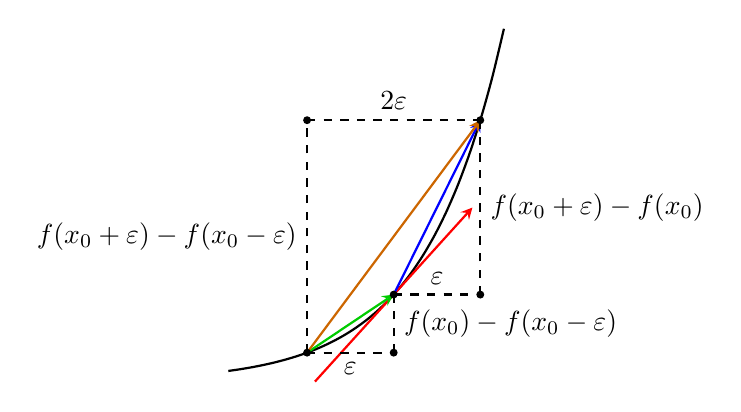
\begin{tikzpicture}[>=stealth, thick]
    % \draw (0, 0) -- ++ (10.5, 0);
    % \draw (0, -1) -- ++ (10.5, 0);
    % \draw (2, 1) -- ++(0, -6);

    % \node [scale = 2] at (1, 0.5) {$x$};
    % \node [scale = 2] at (1, -0.5) {$f'(x)$};
    % \node [scale = 2] at (1, -2.5) {$f(x)$};
    
    % \node [scale = 2] at (2.8, .5) {$-\infty$};
    % \node [scale = 2] at (6, .5) {$1$};
    % \node [scale = 2] at (9.5, .5) {$+\infty$};

    % \node [scale = 2] at (6, -.5) {$0$};
    % \node [scale = 2] at (4, -.5) {$-$};
    % \node [scale = 2] at (8, -.5) {$+$};

    % \node (n1) [scale = 2] at (2.8, -1.5) {$+\infty$};
    % \node (n3) [scale = 2] at (9.2, -1.5) {$+\infty$};
    % \node (n2) [scale = 2] at (5.9, -4.5) {-2};

    % \draw [->] (n1) -- (n2);
    % \draw [->] (n3) -- (n2);


    % graph
    \def\a{1}
    % \begin{scope}[xshift = 14cm, yshift = -3cm, scale = 1.7]
        \draw[domain=-2:1.5,smooth,variable=\x,black] plot ({\x},{exp(\a*\x)});      
        % \node [scale = 2] at (1, 4) {$f(x) = \frac{1}{2}(x-1)^2 - 2$};
        \foreach \xx in {.1}{
            % \draw [fill = black] (\xx, {.5*(\xx - 1)^2 - 2}) circle (1pt);
            \draw[->, red, thick, domain=(\xx-1):(\xx+1),smooth,variable=\x] plot ({\x},{(\a*exp(\a*\xx))*(\x - \xx) + exp(\a*\xx)});      
        }

        % \

        \def\x{.1}
        \def\xp{1.2}
        \def\xm{-1}
        \def\y{{exp(\a*\x)}}
        \def\yp{{exp(\a*\xp)}}
        \def\ym{{exp(\a*\xm)}}

        \draw [->, green!80!black] (\xm, \ym) -- (\x, \y);
        \draw [->, blue] (\x, \y) -- (\xp, \yp);
        \draw [->, orange!80!black] (\xm, \ym) -- (\xp, \yp);

        \draw [dashed] (\xm, \ym) -- node[below] {$\varepsilon$} (\x, \ym);
        \draw [dashed] (\x, \y) -- node[above] {$\varepsilon$} (\xp, \y);
        \draw [dashed] (\x, \ym) -- node[right]{$f(x_0) - f(x_0 - \varepsilon)$} (\x, \y);
        % \draw [dashed] (\xp, \y) -- (\xp, \yp);
        \draw [dashed] (\xp, \y) -- node[right]{$f(x_0 + \varepsilon) - f(x_0)$} (\xp, \yp);


        \draw [dashed] (\xm, \ym) -- node[left]{$f(x_0 + \varepsilon) - f(x_0 - \varepsilon)$} (\xm, \yp);
        \draw [dashed] (\xm, \yp) -- node[above]{$2\varepsilon$} (\xp, \yp);
% 
        % \draw ()
        \draw [fill = black, draw = black] (\x, \y ) circle (1pt);
        \draw [fill = black, draw = black] (\xp, \yp) circle (1pt);
        \draw [fill = black, draw = black] (\xm, \ym) circle (1pt);
        \draw [fill = black, draw = black] (\x, \ym) circle (1pt);
        \draw [fill = black, draw = black] (\xm, \yp) circle (1pt);
        \draw [fill = black, draw = black] (\xp, \y) circle (1pt);


        % \node [scale = 3] at (1, -1.5) {$x^*$};
    % \end{scope}

    % \draw[domain=-3:-2] plot (\x,{(\x-1)*(\x-1)-2}) {[turn] (-3,) coordinate(t1) (-1,0) coordinate(t2)};
    % \draw[domain=-2:2] plot (\x,{(\x-1)*(\x-1)-2});
    % \draw[red] (t1)--(t2);


\end{tikzpicture}
\end{document}